%
%  $Description: Author guidelines and sample document in LaTeX 2.09$
%
%  $Author: ienne $
%  $Date: 1995/09/15 15:20:59 $
%  $Revision: 1.4 $
%

\documentclass[times, 10pt,twocolumn]{article}
\usepackage{latex8}
\usepackage{times}
\usepackage{balance}
\usepackage{epsfig}
\usepackage{graphicx}
%\usepackage{wrapfig}

%\documentstyle[times,art10,twocolumn,latex8]{article}

%-------------------------------------------------------------------------
% take the % away on next line to produce the final camera-ready version
\pagestyle{empty}

%-------------------------------------------------------------------------
\begin{document}

\title{Body Motion Analysis for Multi-Modal Identity Verification}

\author{George Williams  \hspace{0.1in} Graham Taylor \hspace{0.1in} Kirill Smolskiy \hspace{0.1in} Christoph Bregler \\
\emph{Dept. of Computer Science, Courant Institute, New York University}\\
\emph{george,graham,kirill,chris@movement.nyu.edu}\\
% For a paper whose authors are all at the same institution,
% omit the following lines up until the closing ``}''.
% Additional authors and addresses can be added with ``\and'',
% just like the second author.
%\and
%Second Author\\
%Institution2\\
%First line of institution2 address\\ Second line of institution2 address\\
%SecondAuthor@institution2.com\\
}

\maketitle
\thispagestyle{empty}

\begin{abstract}
This paper shows how ``Body Motion Signature Analysis''  -- a new ``soft-biometrics'' technique --  can be used for identity verification.  It is able to extract motion features from the upper body of people and estimates so called ``super-features'' for input to a classifier.  We demonstrate how this new technique can be used to identify people just based on their motion, or it can be used to significantly improve ``hard-biometrics'' techniques.  For example, face verification achieves on this domain 6.45\% Equal Error Rate (EER), and the combined verification performance of motion features and face reduces the error to 4.96\% using an adaptive score-level integration method.  The more ambiguous motion-only performance is 17.1\% EER.

\end{abstract}



%-------------------------------------------------------------------------
\Section{Introduction}
In the past, using motion for recognition has been demonstrated mainly for classifying certain actions or gait styles (\cite{laptevCVPR08,niebles2008unsupervised,efros2003recognizing,DollarPETS05,sarkar2005humanid}).  Using the more ambiguous motion of a person that appears during talking and performing ``body language''  is harder to quantify.  This is similar to what the acoustic speech community calls ``speaker recognition''.  It is not important what the person says, but how it is said.  We developed a new video-based feature extraction technique and methods to train statistical models that classify body motion signatures.  The recognition architecture is inspired by recent progress in speaker recognition research.  
This paper has 3 main contributions: 1) a new visual feature estimation technique,  based on sparse flow computations and motion angle histograms that we call  ``Motion Orientation Signatures'' (MOS).  2) Integration of this new feature into a 3-stage recognition system, 3) a new integration method with a state-of-the-art face recognition architecture \cite{pittpatt}.  This is to the best of our knowledge the first time a system has been demonstrated that can significantly improve a state-of-the-art face recognition system with such complex and ambiguous signals like a person's body-language.


\begin{figure}[bt]
\centering
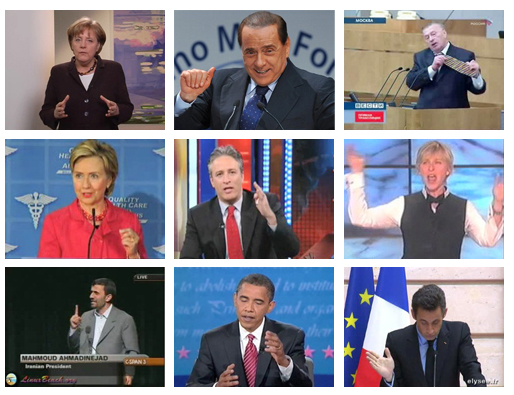
\includegraphics[width=0.96\columnwidth]{matrix_3x3}
\caption{\label{fig_examples}\small Example video frames from our database of people gesturing.
}
\end{figure}
%-------------------------------------------------------------------------
\section{Related Work}
\label{sec_related}
The motion analysis approach in this paper is related to several recent developments.  Human motion has been studied extensively (see \cite{forsyth2005csh} for a survey article).  Tracking body parts explicitly would be of great advantage, but given the low-resolution web footage, it might be impossible to explicitly track. Our technique builds on the observation that it is easy to track just a few reliable features for a few frames (instead over the entire video).   Given those short-term features, we apply an implicit feature representation that compute orientation statistics of local features related to \cite{zelnikmanor2006sad,Dalal06humandetection,laptevCVPR08,niebles2008unsupervised,efros2003recognizing,DollarPETS05}.  Some of these techniques belong to the so called ``Bag-Of-Features'' philosophy, and in section \ref{sec_relatedbag} we will describe details how our approach is different and has superior performance for the new domain of motion style analysis.

Our work is also inspired by recent trends in acoustic speaker recognition.   The simplest techniques apply Gaussian Mixture Models to speech features and the most complex models apply  high-level language model based recognition system \cite{muller2007sci}. Current state-of-the art results are reported  using Support-Vector-Machines applied to super-features \cite{Campbell06supportvector}. Parts of our system are directly inspired by this.
%-------------------------------------------------------------------------
\section{Approach}

As mentioned in section \ref{sec_related}, we are interested in a robust feature detector that does not use explicit tracking or localization (because these techniques fail frequently on low-resolution video).  
\begin{figure}[bt]
\centering
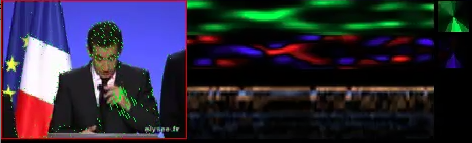
\includegraphics[width=0.96\columnwidth]{Sarkozy_MOS}
%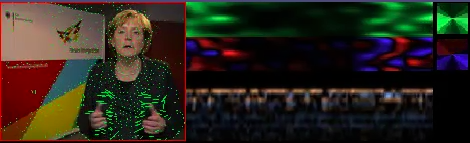
\includegraphics[width=0.96\columnwidth]{Merkel_MOS}
%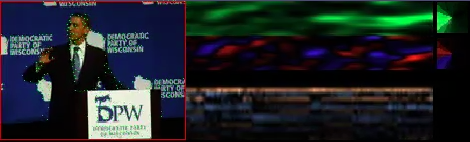
\includegraphics[width=0.96\columnwidth]{Obama_MOS}
%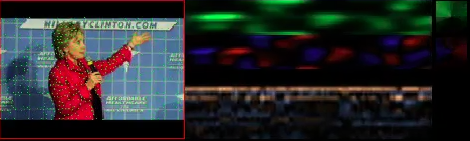
\includegraphics[width=0.96\columnwidth]{Hillary_MOS}
\caption{\label{fig_example_mos} \small Examples of Motion Signatures.  The green colored signature shows how the orientation of the sparse flow features changes over time (top row), and the red-blue color coded signature shows the delta features (middle row).}
\end{figure}
\subsection{MOS: Motion Orientation Signatures}
\label{sec_MOS}
The first step in our extraction schema is flow computation at reliable feature locations  \cite{ST94,bouget:pil}.  Given these robust flow estimates, we compute a weighted histogram discretized into N flow angle bins (we had best experience with N=9). Each angle bin then contains the sum of the flow magnitudes in this direction, i.e. large motions have a larger impact than small motions.  We clip flow magnitudes to be robust to outliers.   The bin values are then blurred across angle bins and across time with a Gaussian kernel ($\sigma=1$ for angles,  $\sigma=2$ for time).  This avoids aliasing effects in the angle discretization and across time.  (Many web-videos are only 15 fps or 24 fps and up-sampled to 30 fps.)  After blurring, we further normalize the histogram values to 0-1 over a temporal window (currently T=10).   This factors out video resolution, camera zoom and body size (double resolution creates double flow magnitudes), but could also factor out important features.  For this reason, we keep the normalization constant as one extra feature. 
As with acoustic speech features, we also compute ``delta-features'', the temporal derivative of each orientation bin value.    Since the bin values are statistics of the visual velocity (flow), the delta-features cover acceleration and deceleration.  

%For example if a subject would clap her hands very fast, it would produce large values in the bin values that cover $90^{O}$ and $270^{O}$ (left and right motion), but also large values in the corresponding delta-features.  If a person just circles her hand with constant velocity, the bin values have large values across all angles, but the delta-features have low values.

Figure \ref{fig_example_mos} shows a few examples that demonstrate what signatures are created with certain video input.  We show several visualizations of these features at http://movement.nyu.edu/GreenDot.

Our initial experiments were done in computing the motion histogram statistics over the entire video frame.  We already showed useful applications of this low-dimensional representation  \cite{breglerICASSP09}. 

\subsection{Face Tracking and Grid based Coarse Locality}
%\begin{wrapfigure}[r]
%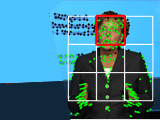
\includegraphics[width=0.45\columnwidth]{matrix_small_merkel2}
%\caption{\label{fig_facegrid} Example of $3 \times 3$ grid for MOS features that is anchored by the face tracker}
%\end{wrapfigure}

We further improved our MOS feature extraction theme in incorporating a state-of-the-art face-tracking system from PittPatt.com \cite{pittpatt} (winner of the 2008 NIST MBGC Challenge), and in coding coarse position information of the MOS features.  This is achieved in placing a $N \times M$ grid of local region of interests (ROIs) around the found face location. The grid is scaled such that it covers the entire possible range of motion of all body parts.  Inside each local ROI of the grid we compute the MOS feature and concatenate all local ROI histograms to one big feature vector.  We achieved highest verification and recognition results with a $5 \times 7$ grid.  We further reduce the dimension of this extended grid feature with PCA.  Best results have been achieved with 32  dimensions.

\subsection{GMM-Super-Features}
\label{sec_superfeat}
We separate the videos into a training and an independent test set of equal size.  For each subject we have video clips from 4 to 8 different dates.   The original collected videos (from YouTube or other sources) are actually longer, sometimes have scene cuts.  The PittPatt face tracker is very robust, and helps us to extract only scenes that have the videos with the subject in the frame.
The video clips are hand labeled with the ground truth (subject name) so we can measure the automatic verification performance for the final system.   In the past there have been many different systems proposed, based on complex architectures, but recent experiments in the speech community (like \cite{Campbell06supportvector}) show that Gaussian Mixture Model (GMM) based Super-Features and Support Vector Machines (SVMs) produce state-of-the-art results.  We also base our video statistics on GMM-Super-Features, although in the future we plan to further investigate more advanced architectures.

A Gaussian Mixture Model is first trained on the entire training database.   128 Gaussians per Mixture Model got best recognition performance.  In speaker recognition, this is called the Universal Background Model (UBM). Given that UBM model, the statistics of each shot are computed in MAP adapting the GMM to the shot \cite{Campbell06supportvector}.  A GMM-Super-Feature is the difference between the UBM mean vectors and the new MAP adapted mean vectors.  If the new video has some unique motion, then at least one mean vector has a large difference to the UBM model.  The GMM-Super-Feature is a fixed-length vector that describes the statistics of the variable length video.   

\subsection{Discriminant Classification}
\cite{Campbell06supportvector}  feed those GMM-Super-Features into a standard SVM classifier, in further scaling the means with the mixing coefficients and covariances of the GMM model:
A linear SVM kernel is a good approximation to the KL-divergence between two utterances.     In \cite{breglerICASSP09} we achieved the best results with such a linear kernel. However we have subsequently found that a logistic regression classifier applied to the GMM-Super-Features achieves the same performance.  All further results reflect logistic regression.
\begin{figure}[bt]
\centering
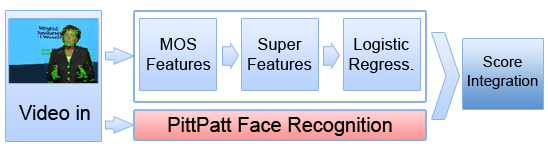
\includegraphics[width=0.96\columnwidth]{fig_arch}
\caption{\label{fig_architecture} \small Multi-Modal Architecture}
\end{figure}


\subsection{Comparison with Bag-Of-Feature Architectures}
\label{sec_relatedbag}
Our approach somewhat is related to so called Bag-Of-Feature architectures used by \cite{laptevCVPR08,niebles2008unsupervised,efros2003recognizing,DollarPETS05} for activity analysis.  We compared\footnote{We plan to include these experiments in a longer technical report} our features and architectural choices element wise with \cite{laptevCVPR08}: 1) When we use so called Space-Time Interest Points (STIP) \cite{laptevCVPR08} instead of our MOS features, we get an relative increase in error 17.1\% to 25\%.  2) We also replaced the GMM-Super-Features with higher-level histograms of vector-quantized codewords, as it is used in all Bag-Of-Feature architectures, and our relative error rate increased further  to 31\% EER.  This is not surprising, since during the vector quantization much information is lost, that is retained by the GMM-Super-Features.
\section{Multi-Modal Experiments}

\begin{figure}[bt]
\centering
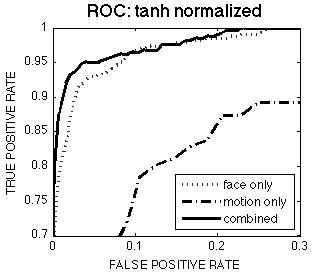
\includegraphics[width=0.96\columnwidth]{roc_tan_normalized}
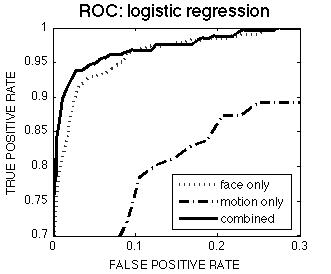
\includegraphics[width=0.96\columnwidth]{roc_logreg}
\caption{\label{fig_results} \small ROC curves using 2 different score integration techniques to combine face recognition and body motion signature recognition results. The combined multi-modal performance is for both integration techniques significant better.}
\end{figure}

Figure \ref{fig_examples}  shows some example video frames from our database.  In total we have 72 minutes of video data with $320 \times 240$ pixel resolution. For each subject we have at least 4 different video clips recorded at different times.   Most subjects are public figures like international politicians or talk show hosts.  We are currently also collecting a database of ``non-famous'' people.

We trained our system to verify if a specific person is present in the video.  As outlined earlier, we first need to train a UBM model and compute GMM super-features for each video clip.  In a final step we trained the logistic regression model. For positive examples we chose two or more videos of that subject, and for negative examples we sampled from the training set part of the remaining videos in our database.  We repeated each experiment 27 times (3 different random initializations for the UBM model, and 9 different verification targets).   Figure \ref{fig_results} shows the ROC curve of our performance.  In the speaker verification community it is common to report the Equal Error Rate EER (the error at the diagonal of the ROC curve, when the number of false positives and false negatives is equal).  For this case we achieved 17.1\%.   

The crucial experiment now is to test if such a soft-biometric modality can be applied in a multi-modal system consisting of other hard-biometrics.  We trained a state-of-the-art face recognition system on the same video database.  Usually face recognition requires high-resolution input images that have at least 90 pixels between the eyes. In our case the eye distance can be as small as 20 pixels.  PittPatt \cite{pittpatt} achieved previously the best face recognition results on video recordings at the NIST MBGC 2008 Challenge.  We trained the PittPatt system on our low-resolution database, and achieved verification performance of 6.45\% EER (figure \ref{fig_results}).  

Previously we experimented with multi-modal integration on the input-level  \cite{breglerICASSP09}.  In this paper we focus on output score-level integration, which allows us to combine several systems that are trained with differently (like PittPatt's face system, and our motion based system).  There are many ways to combine scores \cite{jain2005score}.  We experimented with 1) averaging scores, 2) $\tanh$ normalization \cite{jain2005score}, 3) training another logistic regression on the face and motion scores to predict the multimodal score.  We achieved best results with the $\tanh$ score combination.  This normalizes scores to zero mean and unit variance levels, and applies the $\tanh$ nonlinearity to both normalized scores. It reduced the error relatively by 23\% to 4.96\% EER.  The logistic regression achieved slightly less performance, but still a significant improvement over each modality alone to a combined error of 5.24 \%.  Score averaging, while in some domains very successful did not prove to be useful in this domain (the error increased to 9.62 \%).
\begin{figure}[bt]
\centering
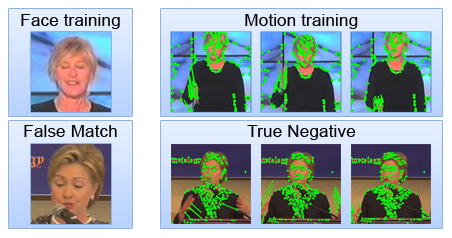
\includegraphics[width=0.96\columnwidth]{fig_example_v2}
\caption{\label{fig_example}\small An example where the face recognition falsely matches a face but the motion system successfully detects a true negative}
\end{figure}
Figure \ref{fig_example} shows an example when the face recognition system by mistake accepts the wrong face, but the motion scores were able to further disambiguate the video to the right classification.


\section{Discussion}
We have demonstrated how the body motion of a subject during speaking and gesturing can be measured and analyzed with a new visual feature extraction technique and methods that have been successfully applied in the speaker recognition community.  Most importantly, we have shown how we can significantly improve the performance of a hard-biometrics system, specifically a state-of-the-art face recognition system with a new soft-biometrics roughly characterized as ``body language''.  This hints strongly that the anecdotal evidence is true: everybody moves in a unique individual way, and we can use this feature for person identification.  Future efforts will be on further improving the visual front end, the score integration techniques, and collection of larger databases.


\section{Acknowledgements}
We would like to thank Peggy Hackney, Ian Spiro, Andreas Stolcke, Yann LeCun, and Rob Fergus for useful discussions and pointers, and the Office of Naval Research (ONR N000140910076, N000140910789).



%-------------------------------------------------------------------------
{\tiny
\bibliographystyle{latex8}
\bibliography{vision}
}
\end{document}

